\documentclass[letterpaper, 12pt]{report}
\usepackage[utf8]{inputenc}
\usepackage[spanish]{babel}
\usepackage{graphicx}
\usepackage[left=4cm, right=2.5cm, top=4cm, bottom=2.5cm]{geometry}
\usepackage{titlesec}
\usepackage{caption}
\usepackage{verbatim}
\usepackage{tocloft}
\usepackage{float}
\usepackage[hidelinks]{hyperref}
\usepackage{apacite}
\usepackage{comment}
\usepackage{amsmath}
\usepackage{parskip}
\usepackage{setspace}
\usepackage{listings}
\usepackage{fancyhdr}

\onehalfspacing %Espacio de 1,5 líneas

\renewcommand{\headrulewidth}{0pt}
\pagestyle{fancy}

\renewcommand{\contentsname}{Índice}

\begin{document}

\begin{titlepage}
  \centering
  \begin{tabular}{@{}p{2cm}@{\hspace{1cm}}p{12cm}@{}}
    \begin{picture}(0,0)
      \put(0,-70){
\includegraphics[width=2cm,height=3cm]{img/logocolor.png}}
    \end{picture}
    &
    \raggedright
    \normalsize UNIVERSIDAD TECNOLÓGICA METROPOLITANA\\
    \normalsize FACULTAD DE INGENIERÍA\\
    \normalsize DEPARTAMENTO DE INFORMÁTICA Y COMPUTACIÓN\\
    \normalsize ESCUELA DE INFORMÁTICA
  \end{tabular}

  \vspace{2.5cm}
  \LARGE \begin{doublespace} MODELO DE APRENDIZAJE AUTOMÁTICO PARA LA PREDICCIÓN DEL COMPORTAMIENTO DE CLIENTES EN CANAL WEB \end{doublespace}
  \vspace{0.1cm}
  \large \begin{singlespace}
    TRABAJO DE TÍTULACIÓN PARA OPTAR AL TÍTULO DE INGENIERO CIVIL EN COMPUTACIÓN MENCIÓN INFORMÁTICA
  \end{singlespace}

  \raggedleft
  \vspace{0.5cm}
  \textbf{\normalsize AUTORES:} \\
  \vspace{0.1cm}
  \normalsize GONZÁLEZ GÁRATE, CRISTÓBAL ANDRES \\
  \vspace{0.1cm}
  \normalsize TAPIA RIQUELME, MARCELO IGNACIO \\
  \vspace{0.1cm}
  \normalsize OYARCE TREJO, DIEGO ESTEBAN \\
  \vspace{0.5cm}
  \textbf{\normalsize PROFESORA GUÍA:} \\
  \normalsize CASTRO OPAZO, PAULA

  \vspace{0.5cm}
  \centering
  \normalsize SANTIAGO - CHILE \\
  \normalsize 2023
\end{titlepage}
\pagenumbering{gobble}

\fancyhf{}

\pagenumbering{roman}
\setcounter{page}{2}
\renewcommand{\thepage}{\roman{page}}

\tableofcontents

\newpage

\begin{singlespace}
  \listoffigures
\end{singlespace}


\setcounter{section}{1}

\chapter{Presentación del proyecto}

\section{Resumen}
El presente documento de Trabajo de Titulación resume exhaustivamente el proceso completo llevado a cabo para desarrollar un modelo de aprendizaje automático capaz de predecir el comportamiento de los usuarios en la nueva plataforma virtual de AFP Capital. Además de detallar la creación de este modelo, se enfoca en la relevancia de la predicción del comportamiento de los clientes y su valor estratégico para las empresas en la actualidad, destacando la importancia de obtener y manejar datos precisos sobre sus comportamientos.

El documento explora varios modelos de aprendizaje considerados como opciones viables, profundizando en la implementación detallada de tres modelos específicos y presentando los resultados obtenidos. Se destaca el proceso de selección del modelo más eficiente entre los evaluados, describiendo minuciosamente este modelo elegido y documentando las pruebas realizadas para demostrar su eficacia final.

Además del desarrollo del modelo, se aborda la creación de un servicio consumible que genera predicciones utilizando el modelo mencionado. Se describe la implementación de una API que facilita la generación de predicciones basadas en los datos de entrada necesarios para el modelo.

El proyecto concluye con la dockerización de todo el trabajo realizado, lo que permite su despliegue simplificado en la plataforma virtual de la empresa. Este enfoque busca garantizar la accesibilidad y la facilidad de implementación del servicio.

Finalmente, se incluyen recomendaciones para mejorar y continuar con el proyecto en caso de que la empresa desee seguir utilizando este modelo. Además, se presentan conclusiones y reflexiones del grupo de trabajo sobre el desarrollo y los hallazgos alcanzados durante el proyecto.

\textbf{Palabras clave:}  Afiliado, Administradora de Fondos de Pensiones, API (Application Programming Interfaces), EDA (Exploratory Data Analysis), Algoritmos de predicción, Algoritmos de clasificación, Modelos de predicción, ETL (Extract, Transform and Load), ARIMA (Modelo de Autorregresión integrada de media móvil), SARIMA (Modelo Estacional de Autorregresión integrada de media móvil), Redes Neuronales Artificiales (ANN), Redes LSTM (Long Short-Term Memory), Redes Neuronales Recurrentes (RNN).

\section{Abstract}
The purpose of this thesis is to show the form and the work plan used throughout the development process of the proposed project. In addition, the results of the research process that has been carried out to date are presented, including studies on customer behavior in web channels, predictive models and algorithms, and how to develop an ETL process.

The main objective of this project is to analyze AFP Capital's customer behavior and usage preferences over a period of up to 6 months, in order to predict future personalized browsing.

The project consists of four phases for its development. The first phase covers the planning and general background for the realization of the project. The second phase focuses on the investigation of the problem under study, based on the current situation. The third phase covers the modeling and development of the project, including the data modeling and ETL process approach. This phase also involves the development of the code that will support and execute the predictive model, through the construction of databases, APIs and testing to mitigate possible errors found. The fourth and last phase concludes the development of the project and focuses on conclusions and recommendations, where the conclusions obtained throughout the process will be presented, and a ...

\textbf{Keywords:} Affiliate, Pension Fund Administrator, API (Application Programming Interfaces), EDA (Exploratory Data Analysis), Predictive Algorithms, Classification Algorithms, Predictive Models, ETL (Extract, Transform and Load).

\clearpage
\pagenumbering{arabic}
\setcounter{page}{1}
\renewcommand{\thepage}{\arabic{page}}


\section{Descripción del trabajo de título}
El trabajo de título se basa en un proyecto que requiere el procesamiento de la data de logs pasados de navegación del sitio web privado de AFP Capital, para detección de comportamientos de clientes y sus preferencias de uso, permitiendo navegaciones futuras customizadas. La lectura de logs será posible gracias a la extracción de dicha información desde Kibana (ElasticSearch), la cual es registrada por APIs variadas que se consumen en el sitio web. Elementos fundamentales del proyecto es el análisis exploratorio de datos, extracciones, transformaciones, cargas, modelo de predicción y detección de preferencias. 

\section{Objetivos}
\subsubsection{Objetivo general}
Analizar el comportamiento de los clientes y sus preferencias de uso en un período igual o inferior a 6 meses, para predecir navegaciones futuras personalizadas. 

\subsubsection{Objetivos específicos }
\begin{itemize}
    \item Realizar una investigación de las herramientas utilizadas para la predicción de comportamiento de usuarios en un canal web.
    \item Llevar a cabo un análisis y estudio de los datos entregados por la empresa. 
    \item Realizar un proceso ETL con la información de navegación web de los clientes de AFP Capital, para analizar su comportamiento dentro del sitio web privado. 
    \item Desarrollar un modelo capaz de predecir el comportamiento de los clientes de AFP Capital, para entregar navegaciones personalizadas futuras.
    \item Establecer recomendaciones de personalización en función de los hallazgos del modelo de predicción para futuras navegaciones dentro del sitio web de AFP Capital.
\end{itemize}

\section{Alcances y Limitaciones}
\subsubsection{Alcances}

El proyecto contempla los siguientes alcances:

\begin{itemize}
\item Se analizará el comportamiento de los clientes de AFP Capital en su nuevo sitio web privado.
\item El proyecto entregará un modelo capaz de predecir el comportamiento de los clientes de AFP Capital en el sitio web, así como una API que permita obtener recomendaciones de comportamiento personalizadas para un afiliado específico.
\end{itemize}

\subsubsection{Limitaciones}

El proyecto tiene las siguientes limitaciones:

\begin{itemize}
\item No se contará con acceso directo a las bases de datos de AFP Capital, por lo tanto, se trabajará con una muestra de datos.
\item No se podrá acceder a información sensible de los clientes de AFP Capital, como los RUTs (Rol Único Tributario) u otra información personal identificable.
\item El análisis se basará únicamente en datos cualitativos de la navegación web de los usuarios.
\end{itemize}

\chapter{La empresa}

\section{Historia}
La historia de AFP Capital se remonta a noviembre de 1980, cuando se implementó en Chile el sistema de pensiones de capitalización individual. El 16 de enero de 1981, se constituyó la sociedad Administradora de Fondos de Pensiones Santa María, que más tarde se transformaría en AFP Capital S.A. Desde sus inicios, la empresa se destacó por su filosofía de servicio, enfocada en satisfacer las necesidades y expectativas de sus afiliados. 
En 1995, AFP Capital estableció la filial Santa María Internacional S.A., con el propósito de expandir su alcance y ofrecer servicios a personas naturales o jurídicas del extranjero, así como invertir en AFP o sociedades relacionadas con materias previsionales en otros países. Esta iniciativa consolidó la presencia de AFP Capital en el ámbito internacional y fortaleció su posición como una administradora de fondos de pensiones líder en la región. 
En el año 2000, se produjo una relevante transacción en la historia de AFP Capital. ING Group adquirió Aetna Inc., incluyendo el 96,56\% de las acciones de AFP Capital S.A. Esta adquisición tuvo como objetivo reforzar la posición de liderazgo de AFP Capital en el mercado previsional chileno y contribuir a su crecimiento y desarrollo. 
Posteriormente, en 2008, AFP Capital llevó a cabo una fusión con AFP Bansander, otra reconocida administradora de fondos de pensiones en Chile. Esta fusión permitió consolidar aún más las operaciones de AFP Capital y fortalecer su presencia en el país. A fines de 2011, Grupo SURA, una empresa líder en el negocio de pensiones en Latinoamérica, adquirió las operaciones de ING en la región. Esta adquisición llevó a AFP Capital a formar parte de Grupo SURA y a beneficiarse de su amplia experiencia y recursos, consolidándose como una compañía destacada en el mercado previsional latinoamericano. En resumen, la historia de AFP Capital está marcada por su constante evolución, consolidación y liderazgo en el mercado de administración de fondos de pensiones en Chile. A lo largo de los años, ha demostrado su compromiso con la excelencia en la prestación de servicios previsionales y su capacidad de adaptación a los cambios y desafíos del entorno económico y regulatorio.

\begin{figure}[H]
    \begin{minipage}[t]{0.9\textwidth}
        \caption{Historia AFP Capital}
        \label{historia-afp}        
    \end{minipage}

    \vspace{10pt}

    \begin{minipage}[b]{1.1\textwidth}
        \centering
        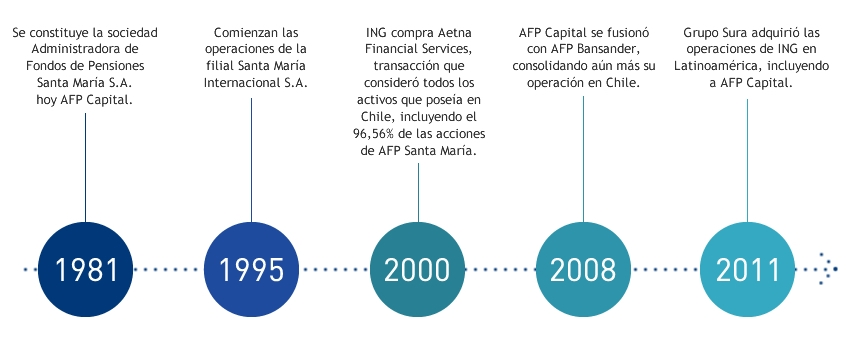
\includegraphics[width=\textwidth]{img/historia-afp-capital.jpg}        
    \end{minipage}

    \begin{minipage}[t]{0.9\textwidth}
        Fuente: AFP Capital. Recuperado de \url{https://www.afpcapital.cl/Quienes-Somos/Paginas/Historia.aspx}
    \end{minipage}
\end{figure}
%agregar la imágen de la historia%

\section{Descripción general}
\input{La empresa/Descripción general}

\section{Misión y visión}
\subsubsection{Misión}
La misión de AFP Capital es: "Acompañamos a nuestros clientes, a través de una asesoría experta y diferenciadora en soluciones de ahorro para alcanzar su número, su Pensión, creciendo sustentablemente, desarrollando a nuestros colaboradores e integrándose responsablemente a la comunidad." \cite{afpcapital} 

\subsubsection{Visión}
La visión de AFP Capital es: "Somos Guías, acompañamos a nuestros clientes a lograr sus sueños a través del ahorro." \cite{afpcapital}

\chapter{Marco teórico}

\section{Importancia de predecir el comportamiento del cliente en un sitio web}
La predicción del comportamiento del cliente dentro de un entorno web se considera a la aplicación de técnicas y modelos analíticos para lograr predecir en cierta manera las posibles necesidades, acciones, preferencias y decisiones que un cliente pueda tomar mientras interactúa en alguna plataforma en línea o sitio web. En los últimos años, ha sido de gran importancia la predicción del comportamiento de los clientes para las empresas, gracias a esto buscan anticipar las necesidades y preferencias de sus clientes, pudiendo adaptar los productos y servicios para entregar una mayor satisfacción al cliente (Zheng, Thompson, Lam, Yoon y Gnanasambandam, 2013). La lealtad de los clientes representa un valor clave para las empresas, ya que un cliente leal seguirá consumiendo los productos y servicios de la empresa, por lo que si se mejora la experiencia del usuario, la satisfacción del cliente aumenta y esto genera un aumento en la ganancia de la empresa. 
Según Zheng, Thompson, Lam, Yoon y Gnanasambandam (2013), la predicción del comportamiento del cliente ayuda a las empresas a identificar oportunidades de mejora y mercado, además de ayudar a tomar decisiones informadas sobre estrategias de publicidad y marketing. El objetivo fundamental de predecir el comportamiento del cliente en un entorno web es lograr comprender y anticipar las acciones de los clientes con la meta de personalizar, mejorar la experiencia de usuario y poder aumentar la satisfacción y fidelidad de los clientes. 
Las predicciones pueden abarcar distintos aspectos del comportamiento de un cliente dentro de un canal web, a grandes rasgos existen 4 tipos de predicciones que se pueden realizar, están las predicciones de compras, donde mediante el análisis de patrones de navegación, su historial de compras, preferencias y características demográficas, gracias a esto se busca predecir las compras futuras de un cliente, se encuentra la predicción de clics, esta busca anticipar los enlaces o elementos con los cuales un cliente va a interactuar dentro de un sitio web, lo que busca mejorar la calidad de contenido que se encuentra desplegado y lograr mejorar la usabilidad del sitio web, también está presente la predicción de abandono de carrito, esta permite tomar acciones de recuperación o retención del cliente, se concentra en identificar aquellos clientes que agregan productos a un carrito de compra pero no finalizan el proceso de compra y por ultimo, esta la predicción de retención de clientes, esta busca predecir qué clientes están más cercanos a abandonar o terminar la relación existente con el sitio web, para poder generar e implementar estrategias para aumentar la fidelización y retención de estos clientes. 



\section{Comportamiento del cliente/afiliado en el canal web}
\subsection{Definición y relevancia del comportamiento del cliente para el negocio}
Considerando los modelos de negocios establecidos por las Administradoras de Fondos de Pensiones [AFP], de ahí radica la importancia de la figura del cliente. Según lo que indica la Real Academia Española, el cliente es la persona que realiza una compra o utiliza los servicios que un profesional o empresa pueda ofrecer (Real Academia Española, s.f), no obstante en base al sistema establecido por las Administradoras de Fondos de Pensiones, el cliente obtiene el nombre de afiliado pues estos contribuyen o se encuentran inscritos en un plan de pensiones (Rasekhi, Fard y Kim, 2016). 
El afiliado es el centro del negocio, cuya gran importancia radica principalmente en la rentabilidad que brinda. Cada trabajador que decida afiliarse se traduce en una ganancia, mientras que cada afiliado que decida desafiliarse genera perdida. Considerando esto es que se puede apreciar la segunda importancia del afiliado, debido a que este promueve la marca si es que la experiencia del servicio de cara al usuario es buena. En tercer lugar, el afiliado, al ser un ganancia para el modelo, este a su vez que obtiene el servicio es capaz de posibilitar el crecimiento de la empresa al tener su preferencia. Por otro lado, la experiencia del cliente y su feedback es valiosa ya que puede brindar conocimiento de los puntos débiles y con posibilidad de mejora que tiene el sistema (Rodriguez, 2023). 
Dentro de las distintas funciones que el cliente tiene, en primer lugar se puede mencionar al cliente como consumidor. Consiste en unas de las funcionalidades más tradicionales puesto que el objetivo intrínseco del cliente es consumir o contratar servicios. Como consumidor es quien adquiere un producto o servicio y lo aprovecha para un fin o necesidad, por lo que la empresa obtiene su principal fuente de ingresos.
En segundo lugar, se tiene al cliente como prosumidor, en otras palabras, consume y produce a la vez (Toffler, 1980). Al momento del consumo, el cliente también deja reseñas o realiza comentarios en lugares especializados, información que resulta de utilidad para generar insights que mejoren la experiencia en el servicio. 
En tercer lugar, se entiende al cliente como crítico, puesto que si la experiencia del cliente es negativa, el feedback y reseñas negativas que este brinde pueden ser de índole constructiva como destructiva. 
En cuarto lugar, se encuentra el cliente como pieza fundamental en el desarrollo de los productos y servicios. Los comentarios de los clientes pueden conducir al desarrollo de servicios innovadores apegados a las necesidades que los clientes indican. Para poder lograr perfeccionar el servicio y productos ofrecidos, es crucial el aporte de los clientes recurrentes o suscriptores del servicio, en el caso específico de las Administradoras de Fondos de Pensiones se refiere a los afiliados. 
En quinto lugar, el cliente como evaluador de la experiencia. Relacionado con los puntos anteriores, la mejor forma de mejorar la experiencia del cliente es tomando en consideración los comentarios de los clientes en esta materia, así se puede generar una diferencia de las otras empresas que constituyen la competencia existente en el mercado. 
Por último, se considera que el cliente puede ser un eventual embajador de la marca, en otras palabras promotores de la misma pudiendo generar recomendaciones, comentarios y reseñas positivas que promuevan el negocio. 


\subsection{Características del comportamiento del cliente en el canal web}
Para comprender la experiencia y el comportamiento del cliente en un canal web, es importante reconocer la existencia del customer journey, el cual describe las distintas etapas por las que un cliente pasa al consumir un producto o servicio. Según \cite{lemon2016customer}, estas etapas incluyen la conciencia, investigación, consideración, compra, uso y evaluación. La etapa de conciencia refiere a la identificación de una necesidad o problema que debe ser resuelto, mientras que la investigación implica la búsqueda de información por parte del cliente para encontrar posibles soluciones y comparar entre diferentes opciones disponibles. Luego, en la etapa de consideración, el cliente evalúa las alternativas y elige la que mejor se adapte a sus necesidades, lo que lleva a la etapa de compra, donde se realiza la contratación o adquisición del servicio seleccionado. Posteriormente, viene la etapa de uso, en la cual el cliente experimenta y evalúa la calidad, funcionalidad y experiencia del servicio. Por último, se encuentra la etapa de evaluación, en la cual el cliente emite un feedback voluntario, tanto positivo como negativo, sobre su experiencia satisfactoria o insatisfactoria. En resumen, las opciones disponibles en el canal web buscan hacer del customer journey una experiencia eficiente y agradable.

En cuanto al segundo párrafo, parece contener información específica sobre el canal web de AFP Capital y las opciones disponibles para los afiliados. Sin embargo, la estructura y organización del texto pueden mejorarse para una mayor claridad. Aquí está el párrafo revisado:

Para acceder al canal web de AFP Capital, es necesario ser afiliado y contar con una cuenta privada personal que incluya el RUT y contraseña. Una vez ingresado al canal web privado, los afiliados tienen a su disposición diversas opciones para satisfacer sus necesidades. Estas incluyen revisión del pago o no de la cotización mensual, la obtención de certificados de cotizaciones, afiliación, antecedentes previsionales y traspaso de fondos, así como certificados tributarios. Además, se pueden obtener certificados generales, como de residencia, suscripción de ahorro previsional voluntario (APV), cuenta 2, remuneraciones imponibles, periodos no cotizados y trabajo pesado. En el caso de afiliados pensionados, también se pueden obtener certificados de asignación familiar, calidad de pensionado, pensiones pagadas, pensión en trámite, ingreso base y comprobante de pago de pensión. Además, es posible acceder a la cartola en línea. El canal web privado permite realizar el ahorro obligatorio y voluntario, inversiones, depósitos directos, consultar planillas de pagos y ver las comisiones cobradas como afiliado. También ofrece la opción de verificar el fondo de pensiones, los tipos de fondos disponibles (A, B, C, D, E) y sus porcentajes de rentabilidad, así como realizar cambios de fondo de pensiones y acceder a educación previsional. Además, se brinda la posibilidad de realizar giros en cuentas personales, acceder a rescates financieros y tramitar la pensión.

\subsection{Factores que afectan el comportamiento del cliente}
%Factores que influyen en el comportamiento del cliente en el canal web, tales como la usabilidad y el diseño del sitio web.
Lemon y Verhoef (2016) proponen que los principales factores que influyen en el comportamiento del usuario y su experiencia son sensoriales, afectivos, cognitivos, puntos de contacto y externos. Dentro de la experiencia sensorial se encuentra lo apreciable con alguno de los sentidos del cuerpo, tanto vista, olor, tacto, entre otros. Respecto de la experiencia afectiva, hay que tener en consideración la emocionalidad del cliente producto de la experiencia del producto o del servicio. Al hablar del aspecto cognitivo, este refiere de los pensamientos, creencias y/o actitudes que el cliente pueda tener respecto de la compañía, el producto o el servicio entregado. Sobre los puntos de contacto, estos hacen mención a las distintas maneras en las que el cliente y la compañía entran en contacto, tales como la publicidad, servicio al cliente, redes sociales o interacciones de tipo transaccional (Lemon y Verhoef, 2016). Por último, el factor externo cuya definición hace referencia a considerar el contexto actual, las condiciones socioeconómicas y otros factores que puedan afectar la experiencia del usuario que se encuentren fuera de control de la compañía. 
Dentro de los factores que pueden influir en el comportamiento de un cliente en el canal web están principalmente, la usabilidad y el diseño. Respecto a la usabilidad, esta depende de 7 características las que garantizan una buena experiencia del usuario. Según Sanchez (2011) la accesibilidad, legibilidad, navegabilidad, facilidad de aprendizaje, velocidad de utilización, eficiencia del usuario y tasas de error del canal web, influyen en la experiencia y posterior feedback que el usuario pueda brindar sobre el uso de los servicios. 
Por otro lado, el diseño del sitio web depende de 5 características para garantizar un buen contenido y estética para lograr que el usuario encuentre lo que busca en el menor tiempo posible, en otras palabras, eficiencia. El autor Walter Sanchez (2011) indica que el diseño debe de ser entendible, novedoso, comprensible, inteligente y atractivo, consiguiendo acercar los contenidos de mejor manera al usuario y logrando conseguir una navegación más intuitiva. Estos factores son de gran importancia para que el usuario pueda encontrar el contenido que busca en el menor tiempo posible y que la experiencia sea positiva al interactuar con la interfaz del sitio web. 


\section{Herramientas para la predicción del comportamiento del cliente en el canal web}

\subsection{Introducción a las herramientas de análisis de datos}
En el entorno empresarial actual, la capacidad de tomar decisiones informadas y basadas en datos se ha vuelto fundamental para el éxito y la competitividad de las organizaciones. El análisis de datos desempeña un papel crucial en este proceso, permitiendo a las empresas obtener información valiosa a partir de grandes volúmenes de datos y utilizarla para comprender el comportamiento del cliente de manera más profunda y precisa. Esto resulta de suma importancia, ya que la calidad de las decisiones tomadas marca la diferencia entre el éxito y el fracaso \cite{analitica-predictiva}.

Dentro de las herramientas de análisis de datos, se destacan cuatro conceptos clave que han revolucionado la forma en que se procesan y se obtiene información de los datos: Business Intelligence, Big Data, Machine Learning y Data Mining. Estas herramientas proporcionan a las empresas la capacidad de extraer conocimientos y patrones significativos de los datos, lo que a su vez les permite tomar decisiones estratégicas más acertadas y personalizar sus estrategias de marketing y atención al cliente.

El Business Intelligence (BI) se refiere a la recopilación, análisis y presentación de datos empresariales para facilitar la toma de decisiones. Mediante el uso de diversas técnicas y herramientas, el BI permite a las empresas visualizar y comprender mejor los datos de sus operaciones y clientes. Esto incluye la generación de informes, el análisis de tendencias, la monitorización de indicadores clave de rendimiento (KPI) y la creación de tableros de control interactivos. El BI ayuda a las organizaciones a identificar oportunidades, detectar áreas de mejora y optimizar su rendimiento en función de datos históricos y en tiempo real. Sobre la inteligencia de negocios, se ha determinado que cada implementación es única para cada proceso empresarial \cite{analitica-empresarial}.

El Big Data se refiere a la gestión y análisis de grandes volúmenes de datos, tanto estructurados como no estructurados, que superan la capacidad de las herramientas tradicionales de almacenamiento y procesamiento. El Big Data se caracteriza por las tres V's: Volumen (gran cantidad de datos), Velocidad (alta velocidad de generación y procesamiento de datos) y Variedad (diversidad de fuentes y formatos de datos). Para aprovechar el potencial del Big Data, las empresas emplean técnicas de procesamiento distribuido y herramientas específicas para el almacenamiento, procesamiento y análisis de estos datos masivos. El análisis de Big Data permite identificar patrones, tendencias y correlaciones ocultas en los datos, lo que brinda información valiosa para entender y anticipar el comportamiento del cliente.

El Machine Learning (aprendizaje automático) es una rama de la inteligencia artificial que permite a los sistemas informáticos aprender y mejorar automáticamente a partir de la experiencia sin ser programados explícitamente. En lugar de basarse en una analítica descriptiva, el Machine Learning ofrece una analítica predictiva \cite{inteligencia-negocios}. Mediante algoritmos y modelos, el Machine Learning permite a las empresas analizar grandes conjuntos de datos y detectar patrones complejos en el comportamiento del cliente. Esto permite realizar predicciones y recomendaciones personalizadas, así como automatizar tareas y procesos, lo que mejora la eficiencia operativa y la experiencia del cliente.

El Data Mining (minería de datos) se refiere al proceso de descubrir información valiosa, patrones y relaciones desconocidas en grandes conjuntos de datos. Utilizando técnicas estadísticas y algoritmos avanzados, el Data Mining permite identificar correlaciones y tendencias ocultas en los datos, lo que ayuda a las empresas a comprender mejor el comportamiento del cliente y tomar decisiones más acertadas. Esta herramienta es especialmente útil para la segmentación de clientes, la detección de fraudes, la recomendación de productos y la personalización de ofertas.


\subsection{Métodos, técnicas y tecnologías de análisis de datos}
En el análisis de datos para predecir el comportamiento del cliente, se utilizan una variedad de métodos, técnicas y tecnologías que permiten procesar y analizar grandes volúmenes de información con el fin de obtener información valiosa. Estas herramientas proporcionan a las empresas y organizaciones la capacidad de comprender mejor a sus clientes, identificar patrones y tendencias, y tomar decisiones estratégicas más acertadas.

Entre los métodos y modelos más utilizados se encuentran la regresión logística, que permite predecir la probabilidad de que un cliente realice una determinada acción o tome una decisión; el clustering, que agrupa a los clientes en segmentos o categorías similares con características y comportamientos comunes; los árboles de decisión, que representan un conjunto de reglas lógicas para clasificar a los clientes en diferentes grupos; el Random Forest, que combina múltiples árboles de decisión para mejorar la precisión de las predicciones; y el Gradient Boosting Machine, que utiliza múltiples modelos de aprendizaje débiles para construir un modelo más robusto y preciso.

Además de los métodos y modelos, existen diversas técnicas que se aplican en el análisis de datos para predecir el comportamiento del cliente. Entre ellas se encuentran las redes neuronales artificiales (ANN), que son modelos inspirados en el funcionamiento del cerebro humano y se utilizan para reconocer patrones y realizar predicciones complejas; y el Support Vector Machine (SVM), que es un algoritmo de aprendizaje automático utilizado para clasificar y predecir datos.

En cuanto a las tecnologías utilizadas en el análisis de datos, se destacan diversas herramientas y lenguajes de programación. Algunas de las más populares son Tableau, que permite visualizar y explorar los datos de manera interactiva; Python, con bibliotecas como Pandas, NumPy y Scikit-learn, que ofrecen una amplia gama de funciones y algoritmos para el análisis de datos; R, con paquetes como dplyr, caret y randomForest, que brindan herramientas estadísticas y de aprendizaje automático; Apache Spark, que permite procesar y analizar grandes volúmenes de datos de manera distribuida; KNIME y RapidMiner, que son plataformas de análisis de datos visuales; y QlikView y Power BI, que son herramientas de visualización de datos y creación de tableros de control.

\subsection{Modelos de predicción de comportamiento del cliente}
\subsubsection{Modelos de regresión}
\noindent
La regresión logística corresponde a un algoritmo de aprendizaje automático supervisado que es empleado para resolver problemas de clasificación. Si bien, su nombre contiene “regresión”, en realidad corresponde a un método de clasificación.

Se da uso a la regresión logística cuando la variable de respuesta o variable objetivo es categórica. En lugar de predecir un valor numérico como en la regresión lineal, la regresión logística estima la probabilidad de que una observación pertenezca a una categoría específica.

Los modelos de regresión logística se basan en la función logística, también conocida como función sigmoide, que mapea cualquier valor real a un rango entre 0 y 1. La función sigmoide tiene la siguiente forma matemática:

\begin{equation*}
    f(z) = \frac{1}{(1 + e^{-z})}
\end{equation*}

En la regresión logística, se ajusta un modelo lineal a los datos de entrada y se aplica la función sigmoide al resultado para obtener la probabilidad de pertenencia a una clase. La ecuación del modelo se expresa como:

\begin{equation*}
    p(y=1|x) = \frac{1}{(1 + e^{(-(b0 + b1x1 + b2x2 + ... + bn*xn))})}
\end{equation*}

Donde:

p(y=1|x) es la probabilidad condicional de que la variable de respuesta sea igual a 1 dada la entrada x.

b0, b1, b2, ..., bn son los coeficientes del modelo que se ajustan durante el proceso de entrenamiento.

x1, x2, ..., xn son los valores de las variables de entrada.

El proceso de ajuste de la regresión logística implica encontrar los mejores valores para los coeficientes del modelo con la finalidad de maximizar la verosimilitud de los datos observados. Esto se puede hacer mediante métodos numéricos como la maximización de la función de verosimilitud o mediante algoritmos de optimización como el gradiente descendente.

Una vez entrenado el modelo, se puede utilizar para hacer predicciones clasificando nuevas observaciones según la probabilidad estimada. Por ejemplo, si la probabilidad estimada de pertenencia a una clase es superior a un umbral (generalmente 0.5), se clasificará como perteneciente a esa clase.

Para nuestro caso en particular, puede ser utilizado el modelo de regresión logística para predecir el comportamiento de usuarios en un canal web, para ello se necesitaría tener datos históricos que contengan información relevante sobre el comportamiento pasado de los usuarios y las variables predictoras asociadas. Estas variables predictoras pueden incluir características demográficas, patrones de uso del sitio web o aplicación, historial de compras, interacciones anteriores, entre otros.

Una vez que se tienen los datos y las variables predictoras, se puede entrenar un modelo de regresión logística utilizando técnicas de ajuste como la maximización de la verosimilitud o el gradiente descendente. Una vez entrenado el modelo, puede ser utilizado para predecir el comportamiento futuro de los usuarios en función de nuevas observaciones o datos entrantes.

Es importante tener en consideración que la calidad de las predicciones dependerá de la calidad de los datos utilizados para entrenar el modelo y de la selección adecuada de las variables predictoras. Además, es fundamental realizar una validación adecuada del modelo utilizando técnicas como la validación cruzada o la separación de conjuntos de entrenamiento y prueba para evaluar su rendimiento y generalización en datos no vistos.

\textbf{Ventajas de los modelos de regresión logística}

\begin{itemize}
    \item Interpretación de resultados: La regresión logística proporciona coeficientes que indican la dirección y la magnitud de la relación entre las variables predictoras y la variable de respuesta. Esto permite interpretar el efecto relativo de cada variable en la probabilidad de pertenecer a una clase específica.
    \item Manejo de variables independientes categóricas: La regresión logística puede manejar tanto variables independientes continuas como categóricas. Incluso puede manejar variables categóricas con más de dos categorías mediante técnicas como la codificación de variables ficticias.
    \item Estimación de probabilidades: La regresión logística estima la probabilidad de pertenencia a una clase específica en lugar de simplemente clasificar observaciones en categorías. Esto es útil cuando se necesita una medida de certeza o riesgo asociado con la clasificación.
    \item Buena capacidad de generalización: La regresión logística puede funcionar bien con conjuntos de datos pequeños o moderados, y es menos propensa al sobreajuste en comparación con otros algoritmos más complejos. Esto la hace adecuada para aplicaciones con muestras limitadas.    
\end{itemize}

\textbf{Desventajas de los modelos de regresión logística}

\begin{itemize}
    \item Linealidad de la relación: La regresión logística asume una relación lineal entre las variables predictoras y la probabilidad logarítmica de la variable de respuesta. Si existe una relación no lineal, la regresión logística puede no ajustarse adecuadamente o requerir transformaciones adicionales de las variables.
    \item Sensible a valores atípicos y datos faltantes: Los valores atípicos o datos faltantes pueden afectar negativamente el rendimiento de la regresión logística. Es necesario manejarlos adecuadamente para evitar sesgos o imprecisiones en los resultados.
    \item Suposición de independencia: La regresión logística asume que las observaciones son independientes entre sí. Si hay dependencias o correlaciones entre las observaciones, la precisión de los resultados puede verse comprometida.
    \item No apto para problemas no lineales: Si existe una relación compleja y no lineal entre las variables predictoras y la variable de respuesta, la regresión logística puede no ser el modelo más adecuado. En tales casos, se pueden requerir técnicas más avanzadas, como modelos no lineales o de aprendizaje profundo.
\end{itemize}
\input{Marco teórico/Herramientas para la predicción del comportamiento del cliente en el canal web/Modelos de predicción/Modelos de recomendación.tex}
\\
Los modelos de series temporales son técnicas utilizadas para analizar y predecir datos secuenciales que están organizados en función del tiempo. En una serie temporal, los datos se registran en intervalos regulares (como horas, días, meses, etc.) y cada punto de datos está asociado con una marca de tiempo.

El objetivo principal de los modelos de series temporales es comprender y capturar los patrones, tendencias y estacionalidad en los datos a lo largo del tiempo, y utilizar esta información para hacer predicciones futuras. Estos modelos son ampliamente utilizados en diversos campos, como la economía, las finanzas, la meteorología, la demanda de productos, la planificación de inventario y más.

Los modelos de series temporales se basan en la suposición de que los datos pasados pueden proporcionar información útil para predecir el futuro. Algunos de los modelos más comunes utilizados en el análisis de series temporales son:
\begin{itemize}
    \item \textbf{Media móvil (MA):} Este modelo estima el valor futuro de la serie temporal en función de un promedio de los errores pasados. Se utiliza para capturar patrones aleatorios o no sistemáticos en los datos.
    \item \textbf{Autoregresión (AR):} Este modelo estima el valor futuro de la serie temporal en función de valores pasados de la propia serie. Se utiliza para capturar la dependencia de la serie en sí misma a lo largo del tiempo.
    \item \textbf{Autoregresión de media móvil (ARMA):} Este modelo combina los enfoques AR y MA para capturar tanto la dependencia de la serie en sí misma como los patrones aleatorios.
    \item \textbf{Autoregresión integrada de media móvil (ARIMA):} Este modelo amplía el modelo ARMA al considerar también las diferencias entre los valores de la serie temporal. Se utiliza para capturar tendencias y estacionalidad en los datos.
\end{itemize}

Además de estos modelos clásicos, también se utilizan enfoques más avanzados, como los modelos de espacio de estados, los modelos de suavizado exponencial y los modelos de redes neuronales recurrentes (RNN), que pueden capturar relaciones más complejas y no lineales en los datos de series temporales.

Es importante destacar que el análisis de series temporales requiere un enfoque cuidadoso para la selección del modelo, la identificación de patrones y la evaluación de la precisión de las predicciones. Además, se deben tener en cuenta factores como la estacionalidad, la estacionariedad de la serie y la presencia de datos faltantes o valores atípicos para obtener resultados confiables.

\begin{itemize}
    \item \textbf{Ventajas de los modelos de series temporales}
    \begin{itemize}
        \item \textbf{Captura de patrones temporales:} Los modelos de series temporales pueden capturar patrones, tendencias y estacionalidad en los datos a lo largo del tiempo. Esto permite comprender mejor la dinámica de los datos y hacer predicciones más precisas.
        \item \textbf{Predicciones a corto plazo:} Los modelos de series temporales son adecuados para hacer predicciones a corto plazo, ya que utilizan la información histórica para predecir los valores futuros. Esto es especialmente útil en aplicaciones donde se necesita anticipar eventos próximos, como demanda de productos o pronóstico del clima.
        \item \textbf{Utilización de datos secuenciales:} Los modelos de series temporales aprovechan la estructura secuencial de los datos y utilizan la información de los puntos anteriores para hacer predicciones en el siguiente punto. Esto permite tener en cuenta la dependencia temporal en los datos y obtener resultados más precisos.
        \item \textbf{Flexibilidad en la elección del modelo:} Existen diferentes tipos de modelos de series temporales que se pueden utilizar según la naturaleza de los datos y los patrones presentes. Esto proporciona flexibilidad para seleccionar el modelo más adecuado para el problema específico.
    \end{itemize}
    \item \textbf{Desventajas de los modelos de series temporales}
    \begin{itemize}
        \item \textbf{Sensibilidad a datos faltantes o valores atípicos:} Los modelos de series temporales pueden verse afectados negativamente por la presencia de datos faltantes o valores atípicos. Estos pueden distorsionar los patrones y afectar la precisión de las predicciones.
        \item \textbf{Dificultad con tendencias no lineales:} Los modelos de series temporales asumen a menudo que las relaciones son lineales o pueden ser capturadas por modelos lineales. Si hay tendencias no lineales en los datos, los modelos lineales pueden no ajustarse adecuadamente y se pueden requerir enfoques más avanzados.
        \item \textbf{Necesidad de datos históricos adecuados:} Los modelos de series temporales requieren una cantidad suficiente de datos históricos para hacer predicciones precisas. En ausencia de datos suficientes, los modelos pueden tener dificultades para capturar patrones y generar resultados confiables.
        \item \textbf{Problemas con cambios estructurales:} Si hay cambios estructurales significativos en los datos de series temporales (por ejemplo, cambios en la estacionalidad o en los patrones), los modelos de series temporales pueden tener dificultades para adaptarse y pueden requerir ajustes manuales.
    \end{itemize}
\end{itemize}
\input{Marco teórico/Herramientas para la predicción del comportamiento del cliente en el canal web/Modelos de predicción/Modelos de atribución.tex}
\\
Los árboles de decisión son modelos de aprendizaje supervisado que se utilizan para predecir a qué clase o categoría pertenece un caso conocido mediante uno o más atributos. Estos modelos se construyen utilizando un algoritmo llamado \emph{partición binaria recursiva}. Durante el entrenamiento, el algoritmo realiza divisiones en un subconjunto de los datos basadas en decisiones asociadas a variables conocidas, generando así dos nuevos subconjuntos. Este proceso se repite de manera recursiva hasta alcanzar un punto de terminación predefinido, lo que resulta en la creación del clasificador basado en árbol de decisión. Luego, cada nuevo dato, que posee atributos conocidos, sigue las ramificaciones del árbol siguiendo las reglas y decisiones generadas durante el proceso de entrenamiento.

En la actualidad, los árboles de decisión son unos de los modelos de aprendizaje más utilizados debido a su buen rendimiento \cite{arboles-decision}. Estos algoritmos pueden generar modelos predictivos tanto para variables cuantitativas (regresión) como para variables cualitativas o categóricas (clasificación).

Como se mencionó anteriormente, un árbol de decisión realiza tareas de clasificación. Un clasificador es un algoritmo que nos permite asignar sistemáticamente una clase a cada uno de los casos presentados.

\begin{figure}[H]
    \begin{minipage}[t]{0.9\textwidth}
        \caption{Estructura de un árbol de decisión}
        \label{arbol-de-decision}        
    \end{minipage}

    \vspace{10pt}

    \begin{minipage}[b]{1.1\textwidth}
        \centering
        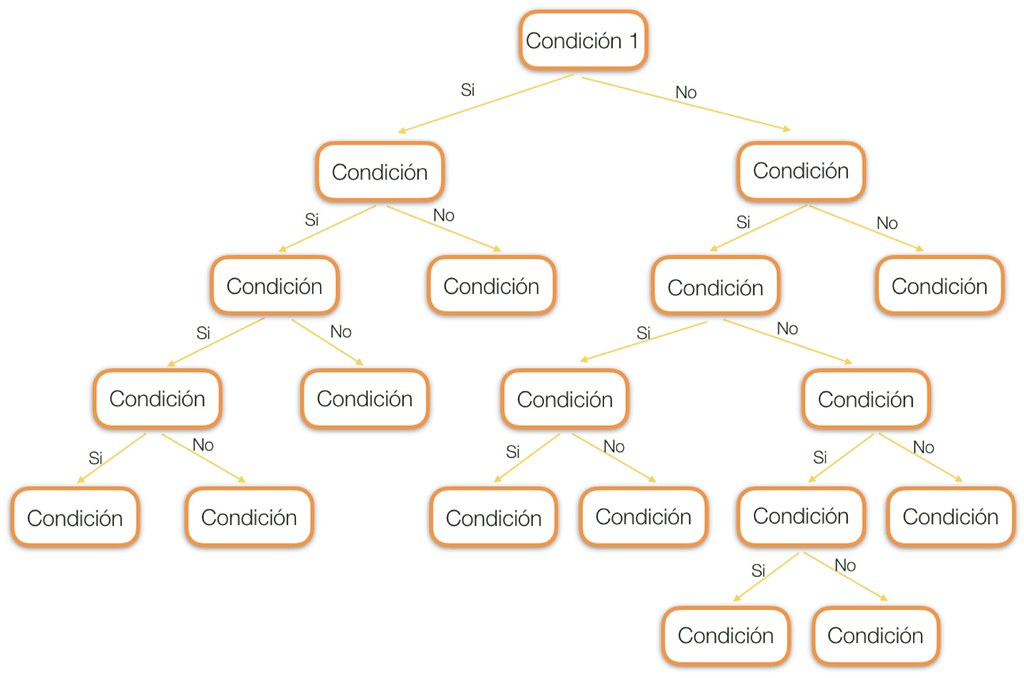
\includegraphics[width=\textwidth]{img/estructura-arbol-de-decision.jpg}        
    \end{minipage}

    \begin{minipage}[t]{0.9\textwidth}
        Fuente: Aprende IA. Recuperado de \url{https://aprendeia.com/arboles-de-decision-clasificacion-teoria-machine-learning/}
    \end{minipage}
\end{figure}

En la figura anterior se puede visualizar la estructura que posee un árbol de decisión, en este se aprecia como actua el algoritmo de partición binaria mencionado al comienzo, tomando un conjunto y separandolo en subconjuntos hasta llegar a un final previamente establecido.

Para estimar la precisión de un clasificador, se calcula la tasa de error de clasificación verdadera. Esta tasa se obtiene evaluando un conjunto de valores X a los que el clasificador asigna una clase incorrecta, y se divide por el total de valores en X. Idealmente, se debería conocer la clase de todos los casos en el universo antes del entrenamiento, o en su defecto, de una muestra de tamaño similar al universo. Sin embargo, en la mayoría de los casos reales, no se dispone de todos los datos del universo, por lo que se trabaja con una muestra y se estima la tasa de error mencionada anteriormente utilizando \emph{estimadores internos}.

\begin{itemize}
    \item \textbf{Ventajas de los árboles de decisión}
    \begin{itemize}
        \item \textbf{Interpretabilidad:} Los árboles de decisión son fácilmente interpretables y comprensibles para los humanos. La estructura del árbol se puede visualizar de manera intuitiva, lo que permite comprender cómo se toman las decisiones y qué atributos son más relevantes para la clasificación.
        \item \textbf{Facilidad de uso:} La construcción y el uso de un árbol de decisión son relativamente sencillos en comparación con otros algoritmos de aprendizaje automático más complejos. No requieren una preparación exhaustiva de los datos ni un procesamiento previo complicado. Además, los árboles de decisión pueden manejar datos numéricos y categóricos sin requerir transformaciones adicionales, lo que simplifica el flujo de trabajo de modelado.
        \item \textbf{Capacidad para manejar datos faltantes y variables irrelevantes:} Los árboles de decisión tienen la capacidad de manejar datos faltantes en los atributos de forma natural. Durante la construcción del árbol, si un atributo tiene valores faltantes, el modelo puede utilizar otros atributos para tomar decisiones sin requerir imputación de datos. Además, los árboles de decisión son resistentes a variables irrelevantes, lo que significa que pueden ignorar atributos que no aportan información útil para la clasificación.
        \item \textbf{Flexibilidad y robustez:} Los árboles de decisión pueden manejar tanto problemas de clasificación como de regresión. Además, son capaces de capturar relaciones no lineales entre los atributos y la variable objetivo. Aunque cada árbol individual puede ser susceptible al sobreajuste, se pueden aplicar técnicas de regularización, como la poda, para mejorar la generalización y evitar el sobreajuste.
        \item \textbf{Eficiencia en tiempo de entrenamiento y predicción:} Los árboles de decisión tienen tiempos de entrenamiento y predicción rápidos, ya que solo implican la evaluación de una serie de reglas de decisión. Aunque el tiempo de construcción puede ser mayor para conjuntos de datos grandes, una vez construido, el árbol puede ser utilizado eficientemente para hacer predicciones en tiempo real.
    \end{itemize}
    \item \textbf{Desventajas de los árboles de decisión}
    \begin{itemize}
        \item \textbf{Sensibilidad a cambios pequeños en los datos:} Los árboles de decisión son muy sensibles a cambios pequeños en los datos de entrenamiento. Una modificación mínima en los datos de entrada puede dar lugar a un árbol de decisión completamente diferente. Esto puede hacer que el modelo sea inestable y su rendimiento pueda variar significativamente.
        \item \textbf{Tendencia al sobreajuste:} Los árboles de decisión tienen la capacidad de adaptarse demasiado a los datos de entrenamiento. Si no se controla adecuadamente, el árbol puede memorizar el ruido o las fluctuaciones aleatorias en los datos de entrenamiento, lo que puede resultar en un mal rendimiento en datos nuevos y no vistos. La poda y otras técnicas de regularización se utilizan para mitigar este problema.
        \item \textbf{Limitaciones en la representación de relaciones complejas:} Aunque los árboles de decisión pueden capturar relaciones no lineales entre atributos y la variable objetivo, pueden tener dificultades para representar relaciones complejas que requieren una combinación de múltiples atributos. Las decisiones tomadas en cada nodo se basan en un solo atributo, lo que puede limitar su capacidad para modelar interacciones más sofisticadas.
        \item \textbf{Propensión a sesgos en los datos de entrenamiento:} Los árboles de decisión pueden verse afectados por sesgos en los datos de entrenamiento, especialmente cuando hay desequilibrios en las clases o falta representación de ciertas categorías. Esto puede resultar en una clasificación desigual o inexacta en casos minoritarios o poco representados.
    \end{itemize}
\end{itemize}
\\
El algoritmo random forest corresponde a un algoritmo empleado en machine learning registrado por Leo Breiman y Adele Cutler \cite{random-forest}, este combina la salida de múltiples árboles de decisión para llegar a un resultado. El uso de random forest se ha hecho popular a causa de su facilidad de uso y flexibilidad, ya que puede ser empleado para problemas de clasificación y regresión.

El random forest se encuentra formado por varios árboles de decisión, los cuales son propensos a tener problemas como sesgos o sobreajuste, pero cuando se trata con una gran cantidad de árboles se logra llegar a resultados más precisos. ''Mientras que los árboles de decisión consideran todas las posibles divisiones de características, los bosques aleatorios solo seleccionan un subconjunto de esas características.'' \cite{random-forest}

Random forest cuenta con tres hiperparámetros principales que se deben de configurar antes de iniciar el entrenamiento \cite{random-forest}:

\begin{itemize}
    \item Tamaño del nodo.
    \item Cantidad de árboles de decisión.
    \item Cantidad de características muestreadas. 
\end{itemize}

El algoritmo se encuentra compuesto de un conjunto de árboles de decisión, cada árbol del conjunto se encuentra compuesto de una muestra de datos, la cual proviene de un conjunto de entrenamiento con reemplazo, llamada muestra de arranque \cite{random-forest}.

A partir de la muestra de entrenamiento, se extrae un porcentaje para reservarlos como datos de prueba, los cuales se conocen como muestra fuera de la bolsa (oob). Luego, se inyecta otra instancia de aleatoriedad mediante el agrupamiento de características, lo que agrega más diversidad al conjunto de datos y reduce la correlación entre los árboles de decisión \cite{random-forest}.

En un Random Forest, el proceso de predicción puede variar según el tipo de problema que se esté abordando \cite{random-forest}. En el caso de tareas de regresión, se utiliza un enfoque de promediado, donde las predicciones de los árboles de decisión individuales se promedian para obtener el valor final de la predicción. Esto proporciona una estimación más precisa y estable del resultado deseado. Por otro lado, en tareas de clasificación, se utiliza un enfoque de votación mayoritaria. Cada árbol de decisión emite su propia predicción y la clase que obtiene la mayoría de votos se selecciona como la clase predicha. Esto permite tomar una decisión conjunta basada en las opiniones de múltiples árboles, lo que puede mejorar la precisión en la clasificación de las muestras.

Finalmente, la muestra extraída en un comienzo, la muestra fuera de la bolsa (oob) será utilizada para realizar una validación cruzada, finalizando la predicción.

\begin{figure}[H]
    \begin{minipage}[t]{0.9\textwidth}
        \caption{Estructura de un random forest}
        \label{random-forest}        
    \end{minipage}

    \vspace{10pt}

    \begin{minipage}[b]{1.1\textwidth}
        \centering
        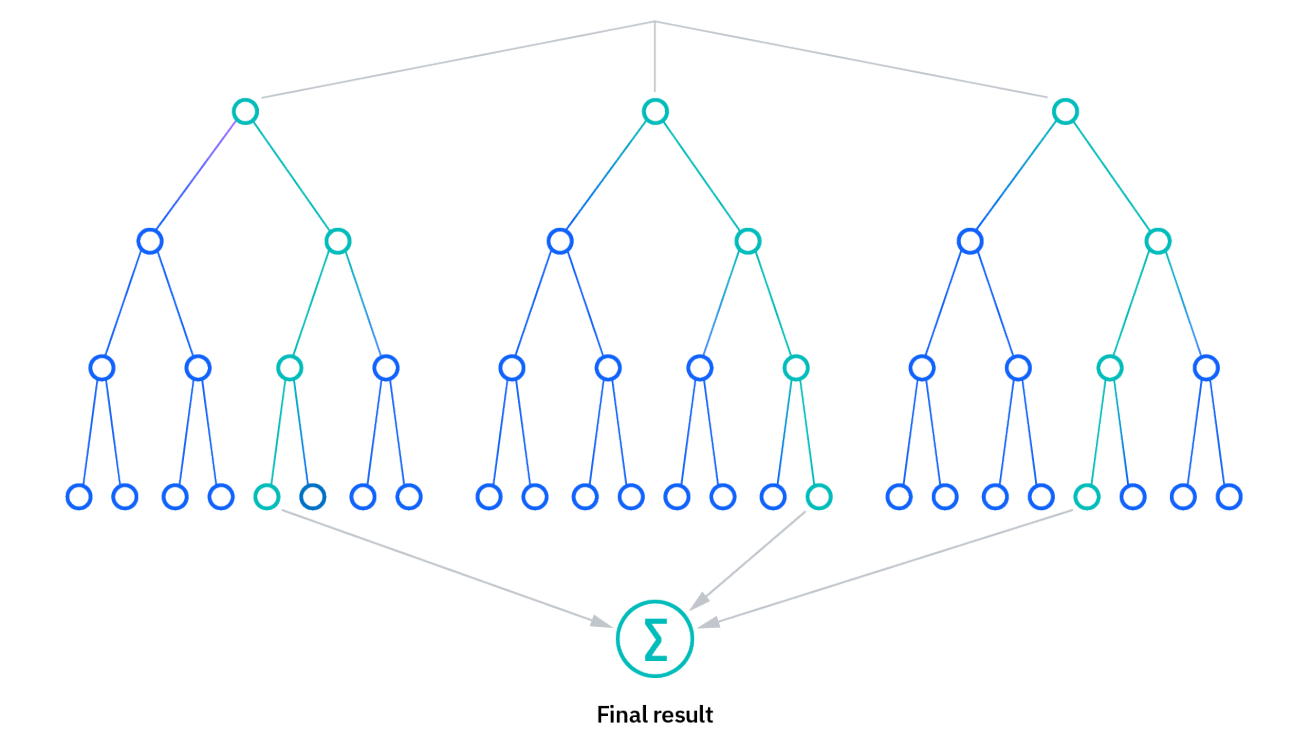
\includegraphics[width=\textwidth]{img/estructura-random-forest.png}        
    \end{minipage}

    \begin{minipage}[t]{0.9\textwidth}
        Fuente: IBM. Recuperado de \url{https://www.ibm.com/mx-es/topics/random-forest}
    \end{minipage}
\end{figure}

\begin{itemize}
    \item \textbf{Ventajas de random forest}
    \begin{itemize}
        \item \textbf{Riesgo reducido de sobreajuste:} Los árboles de decisión corren el riesgo de sobre ajustarse, ya que tienden a ajustar todas las muestras que se encuentran dentro de los datos de entrenamiento. Sin embargo, cuando hay una gran cantidad de árboles de decisión dentro del random forest, el clasificador no será capaz de ajustarse demasiado al modelo, ya que el promedio de los árboles no correlacionados logra reducir la varianza general y el error de predicción.
        \item \textbf{Aporta Flexibilidad:} Debido a su capacidad para abordar con gran precisión tanto tareas de regresión como de clasificación, el método conocido como random forest es ampliamente utilizado por los científicos de datos. Además, su capacidad de agrupar características lo convierte en una herramienta eficaz para estimar valores faltantes, manteniendo la precisión incluso cuando falta parte de los datos.
        \item \textbf{Importancia de la característica fácil de determinar:} El random forest ofrece una forma conveniente de evaluar la importancia o contribución de las variables en un modelo. Existen varias formas de medir la importancia de las características. Por lo general, se utilizan el índice de Gini y la disminución media de impurezas (MDI) para evaluar cuánto afecta la exclusión de una variable específica a la precisión del modelo.
        Sin embargo, otra medida de importancia es la importancia de permutación, también conocida como precisión de disminución media (MDA). La MDA determina la disminución promedio en la precisión al permutar de forma aleatoria los valores de las características en las muestras out-of-bag (muestras que no se utilizan en el proceso de entrenamiento).
    \end{itemize}
    \item \textbf{Desventajas de random forest}
    \begin{itemize}
        \item \textbf{Proceso que requiere mucho tiempo:} Debido a que los algoritmos de random forest son capaces de manejar conjuntos de datos extensos, suelen ofrecer predicciones más precisas. Sin embargo, es importante tener en cuenta que el procesamiento de datos puede volverse lento, ya que se deben calcular los datos para cada árbol de decisión de forma individual.  
        \item \textbf{Requiere más recursos:} Debido a que los random forest procesan conjuntos de datos más grandes, es cierto que se requieren más recursos para almacenar dichos datos. El aumento en el tamaño del conjunto de datos implica una mayor necesidad de memoria y capacidad de almacenamiento para garantizar un funcionamiento eficiente del algoritmo.    
        \item \textbf{Más Complejo:} La interpretación de la predicción de un solo árbol de decisiones resulta más sencilla en comparación con la interpretación de un conjunto de árboles de decisión.
    \end{itemize}
\end{itemize}

\subsection{Tabla comparativa de los modelos de predicción}
La tabla comparativa proporciona información sobre los modelos planteados anteriormente, presentando de forma resumida sus Ventajas, Desventajas y Aplicaciones comunes de los modelos. Permitiendo tener una visión general de las características y consideraciones clave de cada modelo.

\begin{table}[ht]
\captionsetup{font=small} % Ajusta el tamaño de fuente de la leyenda de la tabla
\small % Ajusta el tamaño de fuente de la tabla
\begin{tabular}{|p{0.2\linewidth}|p{0.27\linewidth}|p{0.27\linewidth}|p{0.26\linewidth}|}
\hline
\textbf{Modelo} & \textbf{Ventajas} & \textbf{Desventajas} & \textbf{Aplicaciones} \\
\hline
Modelos de Regresión & 
Proporciona una relación cuantitativa entre variables independientes y la variable de respuesta. & 
Supone una relación lineal entre variables, lo que puede no ser válido en todos los casos. & 
Predicción de valores numéricos continuos. \\
\hline
Modelos de Recomendación & 
Personalización de sugerencias para los usuarios. & 
Puede requerir una gran cantidad de datos y tener problemas con datos faltantes o sesgos inherentes. & 
Recomendaciones de productos en comercio electrónico. \\
\hline
Modelos de Series Temporales & 
Captura patrones temporales y estacionales en los datos a lo largo del tiempo. & 
Sensibilidad a valores atípicos y datos faltantes, y dificultad para capturar tendencias no lineales. & 
Predicción de la demanda de productos. Pronóstico del clima. \\
\hline
Modelos de Atribución & 
Permite cuantificar la contribución relativa de diferentes variables a un resultado o impacto. & 
Puede ser difícil determinar la verdadera relación causal entre las variables. & 
Evaluación del retorno de inversión (ROI) de una campaña publicitaria. \\
\hline
Modelos de Árboles de Decisión & 
Proporciona una estructura de decisiones fácilmente interpretable. & 
Pueden ser propensos al sobreajuste si no se controla adecuadamente. & 
Clasificación y predicción en diversos campos, como medicina, marketing y finanzas. \\
\hline
Modelo Random Forest & 
Combina múltiples árboles de decisión para mejorar la precisión y evitar el sobreajuste. & 
Puede ser computacionalmente costoso y más difícil de interpretar que un solo árbol de decisión. & 
Clasificación y predicción en una amplia gama de aplicaciones, como análisis de datos médicos y detección de fraudes. \\
\hline
\end{tabular}
\end{table}


\subsection{Metodología del proyecto}
Para llevar a cabo el desarrollo del proyecto, se definieron cuatro fases que corresponden a la totalidad del proyecto, las cuales corresponden a:

\subsubsection{Fase 1: Planteamiento y planificación}

Para la primera fase del proyecto, se llevará a cabo una planificación de la manera en la que será abordada la problemática, para desarrollar un anteproyecto que será utilizado para evaluar y planificar las actividades correspondientes al desarrollo del proyecto. Entre ellas se encuentran:

\begin{itemize}
    \item Planteamiento del proyecto y sus objetivos.
    \item Definición de alcances y limitaciones.
    \item Creación de un cronograma de actividades.
\end{itemize}

\subsubsection{Fase 2: Investigación}

Para la segunda fase, se realizará una investigación de herramientas y recursos necesarios para llevar a cabo un diseño de la solución para la problemática del proyecto planteado, sumado a un análisis de las bases de datos brindadas por la empresa AFP Capital. Una vez realizado lo anterior, se llevará a cabo una propuesta de diseño para la problemática, siendo entregada y analizada por la empresa, con la finalidad de pasar a desarrollo. Algunas de las actividades de esta fase corresponden a:

\begin{itemize}
    \item Investigación del problema.
    \item Toma de requerimientos.
    \item Investigación de tecnologías de análisis de datos.
\end{itemize}

\subsubsection{Fase 3: Modelamiento y desarrollo}
Para la tercera fase, se llevará a cabo el diseño y desarrollo del sistema propuesto, además de realizar pruebas para verificar el correcto funcionamiento. Algunas de las actividades de esta fase corresponden a:

\begin{itemize}
    \item Modelado del sistema ETL.
    \item Modelado de la API.
    \item Implementación del modelo propuesto.
    \item Pruebas y validaciones.
    \item Correcciones de errores.
\end{itemize}

\subsubsection{Fase 4: Conclusiones y recomendaciones}
Para la última fase, se dará fin al desarrollo del proyecto, elaborando un manual de usuario el cual indicaría algunas funcionalidades del sistema. Algunas de las actividades de esta fase corresponden a:

\begin{itemize}
    \item Desarrollo de manual de usuario.
    \item Redacción de conclusiones y recomendaciones.
    \item Cierre del proyecto.
\end{itemize}


\subsection{Metodología del sistema}
\subsubsection{CRISP-DM}
La metodología CRISP-DM (Cross-Industry Standard Process for Data Mining) es un proceso estándar utilizado para realizar proyectos de minería de datos. La metodología CRISP-DM se divide en seis fases distintas que se describen a continuación:

\begin{enumerate}
    \item \textbf{Comprensión del problema:} En esta fase se define el problema a resolver y se establecen los objetivos del proyecto. También se recopilan los datos necesarios para el proyecto.
    \item \textbf{Comprensión de los datos:} En esta fase se realiza una exploración de los datos para comprender su calidad, estructura y relevancia para el problema en cuestión.
    \item \textbf{Preparación de los datos:} En esta fase se limpian y procesan los datos para que puedan ser utilizados en la etapa de modelado.
    \item \textbf{Modelado:} En esta fase se aplican técnicas de modelado para desarrollar un modelo predictivo. Se prueban diferentes modelos y se selecciona el que mejor se ajuste a los datos.
    \item \textbf{Evaluación:} En esta fase se evalúa el modelo desarrollado en la fase anterior. Se verifica que el modelo funcione correctamente y se ajuste adecuadamente a los datos.
    \item \textbf{Implementación:} En esta fase se implementa el modelo desarrollado en la fase de modelado en un entorno de producción. También se establecen planes para monitorear el rendimiento del modelo y actualizarlo según sea necesario.
\end{enumerate}

Las fases de la metodología CRISP-DM son iterativas, lo que significa que es posible volver a una fase anterior si es necesario.

\subsubsection{OSEMN}

La metodología OSEMN (acrónimo de las palabras en inglés: Obtain, Scrub, Explore, Model, Interpret) es un proceso utilizado en la minería de datos y el análisis de datos para trabajar con grandes conjuntos de datos de manera efectiva. 

\begin{enumerate}
    \item \textbf{Obtener (Obtain):} En esta etapa, se recopilan los datos necesarios para el análisis. Los datos pueden provenir de diferentes fuentes, como bases de datos, archivos en línea o registros de sensores. La calidad y la cantidad de los datos obtenidos son cruciales para el éxito del análisis.
    \item \textbf{Limpieza (Scrub):} Una vez que se han obtenido los datos, es necesario realizar una limpieza para eliminar datos innecesarios o incorrectos. Esta etapa puede implicar la eliminación de duplicados, la corrección de errores y la eliminación de valores atípicos. El objetivo de esta etapa es obtener datos limpios y coherentes para el análisis.
    \item \textbf{Exploración (Explore):} En esta etapa, se utilizan técnicas de visualización y estadísticas para explorar los datos y obtener información sobre ellos. Se pueden identificar patrones, tendencias y relaciones entre diferentes variables. El objetivo es obtener una comprensión más profunda de los datos y de cómo se relacionan entre sí.
    \item \textbf{Modelado (Model):} En esta etapa, se utilizan técnicas de modelado estadístico o de aprendizaje automático para crear modelos que puedan predecir resultados futuros o identificar patrones en los datos. El objetivo es utilizar los datos para crear un modelo que pueda utilizarse para tomar decisiones informadas.
    \item \textbf{Interpretación (Interpret):} En esta etapa, se interpretan los resultados obtenidos en la etapa de modelado. Los resultados pueden ser utilizados para tomar decisiones o para generar nuevas hipótesis que puedan ser exploradas en futuros análisis.
\end{enumerate}

Se propone el uso de la metodología OSEMN, ya que se enfoca en el análisis de datos y la creación de modelos predictivos. OSEMN también es una metodología más flexible que CRISP-DM, lo que puede ser útil en un proyecto de SCRUM donde se busca una mayor adaptabilidad.

Por otro lado, también se propone el uso de la metodología CRISP-DM, ya que el proyecto incluye una etapa de exploración y análisis de datos, seguida por una fase de construcción de modelos. CRISP-DM se enfoca en el proceso completo de minería de datos, desde la comprensión del problema hasta la implementación del modelo, lo que puede servir para realizar un trabajo más estructurado.

Ya que este proyecto se encuentra bajo el marco de trabajo SCRUM, ambas metodologías pueden ser utilizadas de manera complementaria, utilizando OSEMN para las fases de creación de modelos y CRISP-DM para la etapa de exploración y análisis de datos.


\chapter{Proceso ETL}

\section{Diseño Proceso ETL}
\input{Proceso ETL/Diseño Proceso ETL.tex}

\subsection{Requisitos ETL}
En esta etapa se definen los requisitos del proyecto, las fuentes de datos, los objetivos comerciales y del proceso ETL, las necesidades de análisis y los plazos para realizar el proceso. Estableciendo una base solida para el diseño y buen funcionamiento del proceso ETL.
\begin{itemize}
    \item Fuente de datos: La fuente de datos corresponde a un archivo .CSV que contiene información de la navegación web de los clientes en forma de Web Logs.
    \item Objetivos comerciales: Analizar el comportamiento de los clientes y sus preferencias de uso en un período igual o inferior a 6 meses, para poder predecir navegaciones futuras personalizadas
    \item Objetivos proceso ETL: Realizar las transformaciones necesarias para asegurar que el flujo de datos sea eficiente y preciso, a través de la limpieza de los daotsm normalización, agregación, filtrado, enriquecimiento de datos, cálculos y derivaciones necesarias.
    \item Necesidades de análisis: Realizar un análisis exploratorio de los datos entregados.
\end{itemize}


\subsection{Identificicación fuente de datos}
En esta etapa se determinan las fuentes de datos a ser usadas para el proyecto, incluyendo bases de datos y archivos .CSV y API´s. Esto además comprende la estructura la definición de la estructura, el formato y ubicación de cada fuente de datos dentro del proyecto.


\subsection{Diseño del modelo de datos objetivo}
En esta etapa, se lleva a cabo el diseño del modelo de datos objetivo. Dado el tipo de proyecto, no será necesario crear un modelo multidimensional u algo similar para su implementación. Esto se debe a que los datos de entrada para los algoritmos predictivos consistirán en datos planos, en forma de Dataframes de pandas.

\subsection{Planificación de las transformaciones}
Dentro de esta etapa se realiza la planificación detallada de las transformaciones necesarias para construir una base sólida y consistente para el desarrollo del proyecto. Estas transformaciones implican una serie de pasos que permiten limpiar, filtrar, combinar y enriquecer los datos de manera adecuada.

La planificación de las transformaciones es fundamental para garantizar la calidad y la integridad de los datos que serán utilizados en el proyecto. Durante esta etapa, se identifican las tareas específicas que deben llevarse a cabo para lograr los objetivos establecidos, teniendo en cuenta los requisitos del proyecto y las necesidades del negocio.

Algunas de las transformaciones comunes incluyen \cite{etl-toolkit}:

\begin{itemize}
    \item \textbf{Limpieza de datos:} Se realizan tareas de limpieza para corregir errores, eliminar valores duplicados o inconsistentes, y garantizar la coherencia de los datos. Esto puede incluir la corrección de formatos incorrectos, la normalización de datos, el manejo de valores faltantes o la estandarización de la información. La limpieza se realizo para solo tomar el cuenta los valores no nulos y se establecío el formato 'YYYY;MM;DD;HH;MM;SS.ss' de la columna 'fecha evento'.

    \item \textbf{Filtrado de datos:} Se aplican filtros para seleccionar y extraer los datos relevantes para el proyecto, descartando aquellos que no cumplen con ciertos criterios o condiciones específicas, \textbf{no permitiendo registros sin métodos asociados}. Esto ayuda a reducir el volumen de datos y a enfocarse en la información más relevante y útil.

    \item \textbf{Combinación de datos:} Se integran datos provenientes de diferentes fuentes o fuentes de datos diversas. Esto implica fusionar conjuntos de datos relacionados, realizar uniones o cruces de tablas, y establecer relaciones entre los datos para generar una visión global y coherente.

    \item \textbf{Enriquecimiento de datos:} Se agregan atributos o información adicional a los datos existentes para enriquecer su contexto y mejorar su valor. Esto puede implicar la incorporación de datos externos, la realización de cálculos derivados, la normalización de datos o la aplicación de reglas específicas.
\end{itemize}


Es importante tener en cuenta que la planificación de las transformaciones considera el orden y la secuencia adecuada de ejecución, así como la documentación de cada paso y los criterios de validación y verificación para garantizar la calidad de los datos transformados.
% Por esto es que se diseño el siguiente plan detallado con las transformaciones a aplicar.


\subsection{Selección herramientas}
En esta etapa, se realiza la selección de herramientas de software que se ajusten a las necesidades y requisitos del proyecto para llevar a cabo el proceso ETL de manera eficiente. Se evalúan diferentes opciones disponibles en función de su capacidad, compatibilidad y facilidad de uso, para garantizar una elección adecuada, es por esto que se seleccionaron las siguientes herramientas:
\begin{itemize}
    \item \textbf{Colab}: También conocido como "Colaboratory", permite programar y ejecutar Python en el navegador con las siguientes ventajas \cite{colab}:
    \begin{itemize}
        \item No requiere configuración
        \item Acceso a GPUs sin coste adicional
        \item Permite compartir contenido fácilmente
    \end{itemize}
    Una de las desventajas de usar Colab es que tiene una cantidad de memoria limitada, es decir, si se utiliza el total de memoria disponible no se podrá seguir ejecutando código.
    \item \textbf{Visual Studio Code:} Es un editor de código fuente desarrollado por Microsoft. Es conocido por su enfoque en la simplicidad, la personalización y la eficiencia. Este editor se utilizará en caso de no poder seguir utilizando Colab.
    \item \textbf{Python:} Es un lenguaje de programación interpretado, de alto nivel y de propósito general, conocido por su sintaxis clara y legible. Es utilizado en una amplia gama de aplicaciones, desde desarrollo web hasta ciencia de datos y aprendizaje automático. Python se destaca por su facilidad de aprendizaje y su amplia biblioteca estándar, que ofrece numerosas funcionalidades predefinidas para diversas tareas \cite{python}.
    \begin{itemize}
        \item \textbf{Numpy:} Es una biblioteca fundamental para la computación científica en Python. Proporciona estructuras de datos eficientes y funciones para realizar operaciones numéricas y de manipulación de arrays \cite{numpy}.
        \item \textbf{Pandas:} Es una biblioteca poderosa para el análisis de datos basada en Numpy, que proporciona estructuras de datos flexibles y eficientes, como DataFrames, y un conjunto completo de funciones para la manipulación y transformación de datos \cite{pandas}.
        \item \textbf{Dask:} Es una biblioteca de paralelización flexible que permite escalar el procesamiento de datos en Python. Proporciona estructuras de datos paralelas y operaciones distribuidas que facilitan el procesamiento de grandes volúmenes de datos \cite{dask}.
    \end{itemize}
\end{itemize}


\subsection{Construcción y prueba proceso ETL}
En esta etapa, se lleva a cabo la implementación del diseño del proceso ETL previamente definido, utilizando las herramientas seleccionadas. Se desarrollan los flujos de extracción, transformación y carga de los datos según lo establecido en el diseño.

Una vez implementado, se procede a realizar pruebas exhaustivas para garantizar el correcto funcionamiento del proceso. Estas pruebas incluyen la verificación de la extracción de datos de las fuentes, la correcta aplicación de las transformaciones definidas y la carga exitosa de los datos en el destino final.

El objetivo de las pruebas es asegurar que el proceso ETL cumpla con los requisitos establecidos y que los resultados obtenidos sean los esperados. Esto implica validar la integridad y coherencia de los datos transformados, así como verificar el rendimiento y la escalabilidad del proceso.

En caso de encontrar inconvenientes o desviaciones durante las pruebas, se realizan los ajustes necesarios en el diseño o en la configuración de las herramientas utilizadas. Es fundamental realizar iteraciones y pruebas adicionales hasta obtener resultados consistentes y satisfactorios.

Como primer paso en la construcción del proceso ETL, se importan las bibliotecas pandas y numpy. Luego se le da nombre a las columnas, ya que el contenido del archivo csv solo trae los datos. Una vez nombradas las columnas se ordenan para un entendimiento más facil del conjunto de datos, quedando de la siguiente manera respectivamente: rut, fecha, metodo, canal.

Ahora se comprueba la existencia de valores nulos en el dataframe, resultando lo siguiente:

\begin{figure}[H]
    \begin{minipage}[t]{0.8\textwidth}
        \caption{Valores nulos en el conjunto de datos.}
        \label{valoresNulos}        
    \end{minipage}

    \vspace{10pt}

    \centering
    \begin{minipage}[b]{0.4\textwidth}
        \centering
        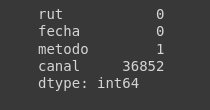
\includegraphics[width=\textwidth]{img/valores-nulos.png}        
    \end{minipage}

    \begin{minipage}[t]{0.9\textwidth}
        Fuente: Elaboración propia.
    \end{minipage}
\end{figure}

Como se puede ver en la imagen anterior solamente los campos 'metodo' y 'canal' poseen valores nulos, de hecho, el primero solo cuenta con un valor nulo. La columna 'canal' cuenta con 36852 valores nulos. Luego de eliminar los valores nulos se pasa a eliminar las filas que contengan métodos inconsistentes, que son:
\begin{itemize}
    \item clientes/surveys
    \item clientes/cuentas/validar-cuenta-corriente
    \item clientes/cuentas/cuentas-bancarias
    \item clientes/cuentas/cuentas-bancarias?rut=81550425
    \item clientes/cuentas/cuentas-bancarias?rut=81691037
    \item clientes/cuentas/cuentas-bancarias?rut=243990041
    \item clientes/cuentas/cuentas-bancarias?rut=12501979K
    \item clientes/cuentas/cuentas-bancarias?rut=169262780
    \item clientes/cuentas/cuentas-bancarias?rut=55022526
    \item clientes/cuentas/cuentas-bancarias?rut=134382953
    \item clientes/cuentas/cuentas-bancarias?rut=126599692
    \item clientes/cuentas/APV/solicitud/giros?rut=151980287\&account=APV
    \item clientes/cuentas/cuentas-bancarias?rut=172165532
\end{itemize}

Al eliminar todas las filas que contengan los métodos antes mencionados se borran un total de 1447 registros. Finalmente, se eliman un total de 38299 filas del dataset original.

\subsection{Monitoreo proceso ETL}
Se establece un sistema de monitoreo para poder supervisar el rendimiento del proceso ETL, logrando identificar posibles problemas y garantizar la calidad de los datos. Es en esta etapa donde se hace un mantenimiento del proceso, pudiendo tener actualizaciones de las transformaciones, resolución de problemas y optimizar el proceso.

\chapter{Exploratory Data Analysis (EDA)}

\section{Introducción al EDA}
%Breve descripción del objetivo del análisis exploratorio de datos.
%Explicación de la importancia de comprender los datos antes de construir el modelo de predicción de comportamiento de los clientes.
El análisis exploratorio de datos (EDA, por sus siglas en inglés, Exploratory Data Analysis) es una fase fundamental en la investigación y comprensión de un conjunto de datos. Como su nombre lo indica, el EDA tiene como objetivo explorar y examinar los datos de manera detallada, utilizando resúmenes numéricos y visuales, con el fin de descubrir patrones, tendencias y características no anticipadas. Es considerado uno de los primeros pasos en el proceso de análisis, ya que proporciona una visión general de los datos antes de realizar un análisis más profundo \cite{ruiz2022exploratorio}.

El enfoque principal del EDA radica en el uso de herramientas y técnicas visuales y gráficas para revelar información clave sobre los datos en estudio \cite{parra2002exploratorio}. Estas técnicas incluyen el diagrama de tallo y hoja, el diagrama de caja y bigotes, y el diagrama de dispersión, entre otros. Al aplicar estas técnicas de análisis gráfico, podemos obtener una comprensión más profunda de la distribución y estructura de los datos, así como identificar relaciones entre las variables de interés. Además, el EDA nos brinda la capacidad de detectar posibles errores o puntos extremos, como anomalías, que podrían afectar la calidad de los resultados del análisis.

Los beneficios clave del análisis exploratorio de datos son los siguientes:
\begin{itemize}
    \item \textbf{Conocer la distribución y estructura de los datos:} El EDA nos permite examinar la distribución de las variables y comprender cómo se organizan y dispersan los datos en el conjunto. Esto es fundamental para seleccionar las técnicas adecuadas de análisis estadístico y modelado.
    \item \textbf{Estudiar la relación entre variables:} Mediante el análisis de correlación y la visualización de patrones en los diagramas de dispersión, podemos explorar las relaciones entre las variables y comprender cómo interactúan entre sí. Esto nos brinda información valiosa para identificar posibles dependencias y tendencias en los datos.
    \item \textbf{Encontrar posibles errores y anomalías:} El EDA nos ayuda a identificar valores atípicos, datos faltantes u otros errores en los datos. Estas anomalías pueden tener un impacto significativo en los resultados del análisis, por lo que es importante detectarlas y tratarlas de manera adecuada.
\end{itemize}

\section{Recopilación de datos}
Los datos recopilados de los registros de navegación de los afiliados de AFP Capital constituyen una valiosa fuente de información para comprender el comportamiento y las preferencias de los usuarios en la plataforma web. Estos registros nos permiten analizar cómo interactúan los afiliados con los diferentes canales y métodos disponibles, así como realizar un seguimiento detallado de las fechas y horarios en que se llevan a cabo estas interacciones.

El dataset inicial entregado para este proyecto cuenta con 58,252 registros de navegación de usuarios, lo cual proporciona una cantidad significativa de información para su análisis. Antes de utilizar estos datos, se realizó un proceso de anonimización para proteger la privacidad de los usuarios, específicamente modificando el campo del rut para no mostrar el dato original. De esta manera, se garantiza que los registros sean tratados de forma confidencial y segura.

Los cuatro campos principales que conforman el conjunto de datos son el rut, la fecha del evento, el método y el canal. El rut, que ha sido modificado, actúa como un identificador único para cada usuario y permite realizar análisis individuales sin revelar su identidad. La fecha del evento registra el momento exacto en que se llevó a cabo cada navegación, lo cual es crucial para identificar patrones y tendencias a lo largo del tiempo. El campo del método describe la interacción específica realizada por el usuario en el canal correspondiente, proporcionando información detallada sobre las acciones que realizan. Por último, el campo del canal indica el sitio o ambiente particular en el cual tuvo lugar cada interacción, lo que puede ser útil para comprender las preferencias de los usuarios en relación con los diferentes entornos disponibles.

Con respecto al preprocesamiento de datos realizado hasta la fecha, se ha seguido el proceso ETL (Extracción, Transformación y Carga) que se describe en detalle en el capítulo anterior. Este proceso implica extraer los datos de las fuentes de origen, transformarlos en un formato adecuado y cargarlos en un sistema de almacenamiento para su posterior análisis. Se utilizaron diversas herramientas especializadas para llevar a cabo estas tareas, asegurando la calidad y coherencia de los datos procesados.

Es importante destacar que, si bien los datos recopilados ofrecen una valiosa perspectiva sobre el comportamiento de los usuarios en la plataforma web, es necesario tener en cuenta que existe un sesgo en la muestra de datos. En particular, los registros de navegación corresponden principalmente a afiliados con rentas altas. Esto implica que los usuarios con ingresos más altos, aquellos que cotizan por un valor elevado o el valor máximo, están sobrerrepresentados en la muestra. Por lo tanto, al interpretar y generalizar los resultados obtenidos, es fundamental tener en cuenta esta limitación y considerar posibles variaciones en el comportamiento de otros segmentos de usuarios.

\section{Estadísticas descriptivas}
Resumen de las principales estadísticas descriptivas de las variables relevantes en los logs de navegación.
Análisis de la distribución de los datos, incluyendo medidas de centralidad y dispersión.
Haciendo uso de la librería pandas podemos obtener informacion respecto al dataframe, cantidad de valores únicos y calcular estadísticas descriptivas:

Podemos obtener informacion respecto a la cantidad de valores faltantes de cada dataframe que se está utilizando, los cuales son \textbf{36853}:

\begin{figure}[H]
    \begin{minipage}[t]{0.9\textwidth}
        \caption{Datos faltantes dataframes.}
        \label{descripcion_dataframe}        
    \end{minipage}

    \vspace{10pt}

    \begin{minipage}[b]{0.85\textwidth}
        \centering
        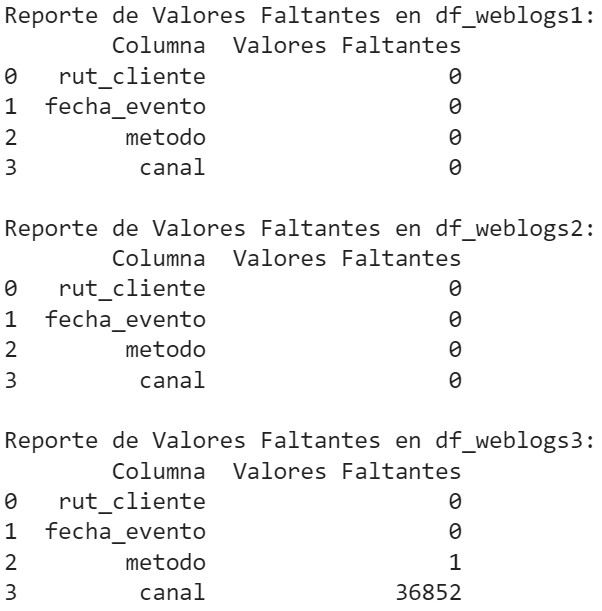
\includegraphics[width=\textwidth]{img/valores faltantes datasets.jpg}        
    \end{minipage}

    \begin{minipage}[t]{0.9\textwidth}
        Fuente: Elaboración propia.
    \end{minipage}
\end{figure}

\begin{itemize}
    \item \textbf{rut cliente:} Contiene datos de tipo int64.
    \item \textbf{fecha evento:} Contiene datos de tipo object.
    \item \textbf{metodo:} Contiene datos de tipo object.
    \item \textbf{canal:} Contiene datos de tipo object.
\end{itemize}

Además se puede conocer la cantidad de valores únicos que posee cada una de las columnas de los 2 datasets:

Dataset 1:

\begin{itemize}
    \item \textbf{rut cliente:} Contiene 40125 valores únicos.
    \item \textbf{fecha evento:} Contiene 80181 valores únicos.
    \item \textbf{metodo:} Contiene 81254 valores únicos.
    \item \textbf{canal:} Contiene 81254 valores únicos.
\end{itemize}

Dataset 2:

\begin{itemize}
    \item \textbf{rut cliente:} Contiene 40224 valores únicos.
    \item \textbf{fecha evento:} Contiene 80470 valores únicos.
    \item \textbf{metodo:} Contiene 81546 valores únicos.
    \item \textbf{canal:} Contiene 81546 valores únicos.
\end{itemize}

La librería pandas ofrece una buena cantidad de estadísticas descriptivas gracias a su función .describe, las cuales se muestran a continuación:
\begin{itemize}
    \item \textbf{Recuento (count):} Calcula el número de valores no nulos en cada columna. \textbf{count: 58009.000000} valores no nulos.
    \item \textbf{Media (mean):} Calcula la media de las columnas numéricas. \textbf{mean: 504.854902} 
    \item \textbf{Desviación estándar (std):} Calcula la desviación estándar de las columnas numéricas. \textbf{std: 553.964179}
    \item \textbf{Mínimo (min):} Calcula el valor mínimo de las columnas numéricas. \textbf{min: 1.000000}
    \item \textbf{Cuartiles:} Calcula los cuartiles de las columnas numéricas 
    \begin{itemize}
        \item \textbf{25\%: 8.000000}
        \item \textbf{50\%: 303.000000}
        \item \textbf{75\%: 884.000000}
    \end{itemize}
    \item \textbf{Máximo (max):} Calcula el valor máximo de las columnas numéricas. \textbf{max: 1815.000000}
\end{itemize}
%Identificación de cualquier valor atípico o dato faltante en los registros y discusión sobre cómo se manejarán estos casos.

% \subsection{Visualizaión de datos}
% Utilización de gráficos y visualizaciones para explorar los datos.
Representación visual de las características relevantes de los clientes y su comportamiento en el canal web.



%Análisis de patrones, tendencias o relaciones identificadas a través de las visualizaciones.

%\subsection{Análisis de correlación}
%%Exploración de la relación entre las variables relevantes en los logs de navegación.
%Cálculo de coeficientes de correlación u otras medidas para evaluar la fuerza y dirección de las relaciones.
%Interpretación de los resultados obtenidos y discusión sobre cómo pueden influir en el modelo de predicción.

%\subsection{Análisis de variables importantes}
%%Identificación de las variables más relevantes o influyentes en el comportamiento de los clientes.
%Uso de técnicas estadísticas o algoritmos de selección de características para determinar la importancia relativa de las variables.
%Discusión de los hallazgos y cómo se utilizarán en el modelo de predicción.

%\subsection{Resultados}
%%Resumen de los principales hallazgos del análisis exploratorio de datos.
%Discusión de las implicaciones de estos hallazgos en el proyecto de %empresa y el modelo de predicción de comportamiento de los clientes.
%Posibles limitaciones del análisis exploratorio y propuestas de futuras investigaciones.

\begin{doublespace}
  \bibliographystyle{apacite}
  \bibliography{Bibliografia}
\end{doublespace}

\end{document}